\chapter{2 Samuel 20}

\begin{figure}
  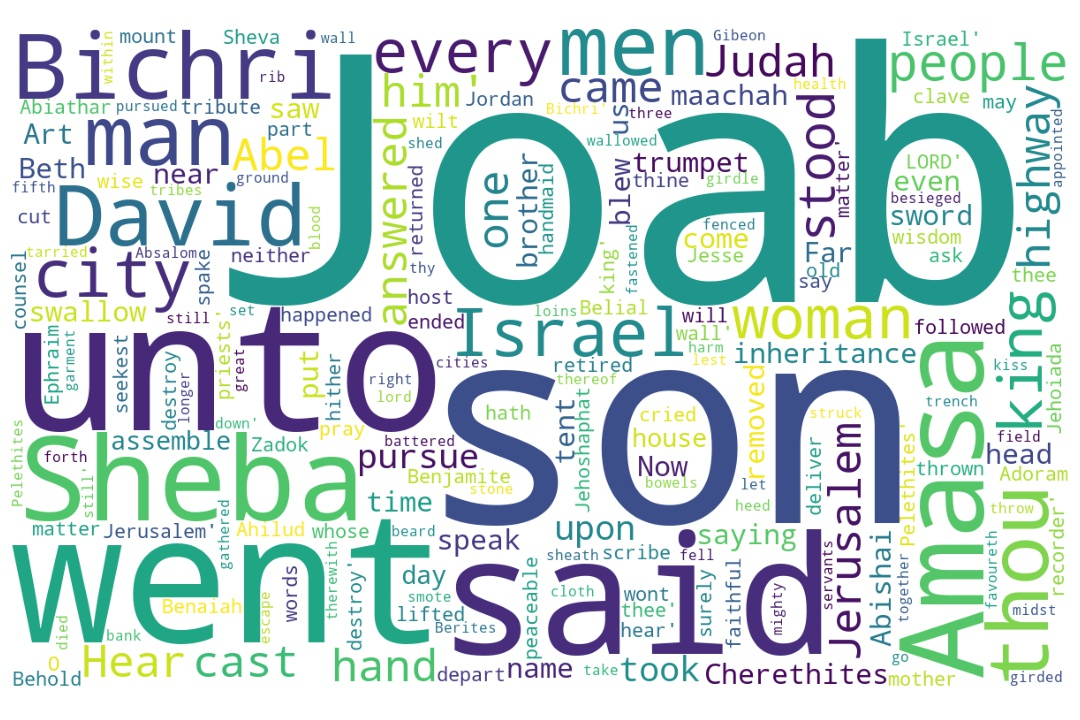
\includegraphics[width=\linewidth]{10OT-2Samuel/2Samuel20-WordCloud.jpg}
  \caption{1 Samuel 20 Word Cloud}
  \label{fig:1 Samuel 20 Word Cloud}
\end{figure}

%%%%%%%%%%%%%%%%%%%%%%%%%%%%%%%%%%%%%%%%%
%%%%%%%%%%%%%%%%%%%%%%%%%%%%%%%%%%%%%%%%%

\marginpar{\scriptsize \centering \fcolorbox{bone}{lime}{\textbf{CONFLICT \& CHARACTER}}\\ (2 Samuel 20:1-26) \begin{compactenum}[I.][8]
   \item The  \textbf{Next} Revolt \index[scripture]{2Samuel!2Sa 20:01} (2Sa 20:1) 
   \item The  \textbf{Northern} Hostility \index[scripture]{2Samuel!2Sa 20:02} (2Sa 20:2) 
   \item A  \textbf{Nasty} Ambush \index[scripture]{2Samuel!2Sa 20:10} (2Sa 20:10) 
   \item A  \textbf{Narrow} Mind \index[scripture]{2Samuel!2Sa 20:11} (2Sa 20:11) 
   \item A  \textbf{Necessary} Judgment \index[scripture]{2Samuel!2Sa 20:22} (2Sa 20:22) 
   \item  \textbf{Named} Officials \index[scripture]{2Samuel!2Sa 20:23--26} (2Sa 20:23--26) 
   \item A  \textbf{Notable} Contradiction -- David's disdain for men like Joab, yet dependence on them (see \index[scripture]{2Samuel!2Sa 19:22} 2Sa 19:22) 
\end{compactenum}}

\footnote{\textcolor[cmyk]{0.99998,1,0,0}{\hyperlink{TOC}{Return to end of Table of Contents.}}}\footnote{\href{https://audiobible.com/bible/2_samuel_20.html}{\textcolor[cmyk]{0.99998,1,0,0}{2 Samuel 20 Audio}}}\textcolor[cmyk]{0.99998,1,0,0}{And there happened to be there \fcolorbox{bone}{bone}{a} man of Belial, whose name \emph{was} Sheba, the son of Bichri, \fcolorbox{bone}{bone}{a} Benjamite: and he blew \fcolorbox{bone}{bone}{a} trumpet, and said, We have \fcolorbox{bone}{lime}{no part in David}, neither have we inheritance in the son of Jesse: every man to his tents, O Israel.}
[2] \textcolor[cmyk]{0.99998,1,0,0}{So every man of Israel went up from after David, \emph{and} \fcolorbox{bone}{lime}{followed Sheba} the son of Bichri: but the men of Judah clave unto their king, from Jordan even to Jerusalem.}\\
\\
\P \textcolor[cmyk]{0.99998,1,0,0}{And David came to his house at Jerusalem; and the king took the ten women \emph{his} concubines, whom he had left to keep the house, and put them in ward, and fed them, but went not in unto them. So they were shut up unto the day of their death, living in widowhood.}\\
\\
\P \textcolor[cmyk]{0.99998,1,0,0}{Then said the king to Amasa, Assemble me the men of Judah within three days, and be thou here present.}
[5] \textcolor[cmyk]{0.99998,1,0,0}{So Amasa went to assemble \emph{the} \emph{men} \emph{of} Judah: but he tarried longer than the set time which he had appointed him.}
[6] \textcolor[cmyk]{0.99998,1,0,0}{And David said to Abishai, Now shall Sheba the son of Bichri do us more harm than \emph{did} Absalom: take thou thy lord's servants, and pursue after him, lest he get him fenced cities, and escape us.}
[7] \textcolor[cmyk]{0.99998,1,0,0}{And there went out after him Joab's men, and the Cherethites, and the Pelethites, and all the mighty men: and they went out of Jerusalem, to pursue after Sheba the son of Bichri.}
[8] \textcolor[cmyk]{0.99998,1,0,0}{When they \emph{were} at the great stone which \emph{is} in Gibeon, Amasa went before them. And Joab's garment that he had put on was girded unto him, and upon it \fcolorbox{bone}{bone}{a} girdle \emph{with} \fcolorbox{bone}{bone}{a} sword fastened upon his loins in the sheath thereof; and as he went forth it fell out.}
[9] \textcolor[cmyk]{0.99998,1,0,0}{And Joab said to Amasa, \emph{Art} thou in health, my brother? And Joab took Amasa by the beard with the right hand to kiss him.}
[10] \textcolor[cmyk]{0.99998,1,0,0}{But Amasa took no heed to the sword that \emph{was} in Joab's hand: so he \fcolorbox{bone}{lime}{smote him} therewith in the fifth \emph{rib}, and shed out his bowels to the ground, and struck him not again; and he died. So Joab and Abishai his brother pursued after Sheba the son of Bichri.}
[11] \textcolor[cmyk]{0.99998,1,0,0}{And one of Joab's men stood by him, and said, He that favoureth Joab, and he that \emph{is} for David, \emph{let} \emph{him} \fcolorbox{bone}{lime}{\emph{go} after Joab}.}
[12] \textcolor[cmyk]{0.99998,1,0,0}{And Amasa wallowed in blood in the midst of the highway. And when the man saw that all the people stood still, he removed Amasa out of the highway into the field, and cast \fcolorbox{bone}{bone}{a} cloth upon him, when he saw that every one that came by him stood still.}
[13] \textcolor[cmyk]{0.99998,1,0,0}{When he was removed out of the highway, all the people went on after Joab, to pursue after Sheba the son of Bichri.}\\
\\
\P \textcolor[cmyk]{0.99998,1,0,0}{And he went through all the tribes of Israel unto Abel, and to Beth-maachah, and all the Berites: and they were gathered together, and went also after him.}
[15] \textcolor[cmyk]{0.99998,1,0,0}{And they came and besieged him in Abel of Beth-maachah, and they cast up \fcolorbox{bone}{bone}{a} bank against the city, and it stood in the trench: and all the people that \emph{were} with Joab battered the wall, to throw it down.}\\
\\
\P \textcolor[cmyk]{0.99998,1,0,0}{Then cried \fcolorbox{bone}{bone}{a} wise woman out of the city, Hear, hear; say, I pray you, unto Joab, Come near hither, that I may speak with thee.}
[17] \textcolor[cmyk]{0.99998,1,0,0}{And when he was come near unto her, the woman said, \emph{Art} thou Joab? And he answered, I \emph{am} \emph{he}. Then she said unto him, Hear the words of thine handmaid. And he answered, I do hear.}
[18] \textcolor[cmyk]{0.99998,1,0,0}{Then she spake, saying, They were wont to speak in old time, saying, They shall surely ask \emph{counsel} at Abel: and so they ended \emph{the} \emph{matter}.}
[19] \textcolor[cmyk]{0.99998,1,0,0}{I \emph{am} \emph{one} \emph{of} \emph{them} \emph{that} \emph{are} peaceable \emph{and} faithful in Israel: thou seekest to destroy \fcolorbox{bone}{bone}{a} city and \fcolorbox{bone}{bone}{a} mother in Israel: why wilt thou swallow up the inheritance of the LORD?}
[20] \textcolor[cmyk]{0.99998,1,0,0}{And Joab answered and said, Far be it, far be it from me, that I should swallow up or destroy.}
[21] \textcolor[cmyk]{0.99998,1,0,0}{The matter \emph{is} not so: but \fcolorbox{bone}{bone}{a} man of mount Ephraim, Sheba the son of Bichri by name, hath lifted up his hand against the king, \emph{even} against David: deliver him only, and I will depart from the city. And the woman said unto Joab, Behold, his head shall be thrown to thee over the wall.}
[22] \textcolor[cmyk]{0.99998,1,0,0}{Then the woman went unto all the people in her wisdom. And they \fcolorbox{bone}{lime}{cut off the head} of Sheba the son of Bichri, and cast \emph{it} out to Joab. And he blew \fcolorbox{bone}{bone}{a} trumpet, and they retired from the city, every man to his tent. And Joab returned to Jerusalem unto the king.}\\
\\
\P \textcolor[cmyk]{0.99998,1,0,0}{Now \fcolorbox{bone}{lime}{Joab} \emph{was} over all the host of Israel: and \fcolorbox{bone}{lime}{Benaiah} the son of Jehoiada \emph{was} over the Cherethites and over the Pelethites:}
[24] \textcolor[cmyk]{0.99998,1,0,0}{And \fcolorbox{bone}{lime}{Adoram} \emph{was} over the tribute: and Jehoshaphat the son of Ahilud \emph{was} recorder:}
[25] \textcolor[cmyk]{0.99998,1,0,0}{And \fcolorbox{bone}{lime}{Sheva} \emph{was} scribe: and \fcolorbox{bone}{lime}{Zadok} and \fcolorbox{bone}{lime}{Abiathar} \emph{were} the priests:}
[26] \textcolor[cmyk]{0.99998,1,0,0}{And \fcolorbox{bone}{lime}{Ira} also the Jairite was \fcolorbox{bone}{bone}{a} chief ruler about David.}